\documentclass{article}
\usepackage{graphicx} % Required for inserting images

\title{Swetify}
\author{Niccolò Malgeri, Filippo Viti, Alessio Delli Colli}
\date{July 2024}

\begin{document}

\maketitle

\tableofcontents
\newpage


\section{Motivazioni}
Il nostro intensivo utilizzo di piattaforme di streaming musicali ha suscitato in noi un interesse riguardo
la loro struttura e il desiderio di replicarne il funzionamento.\\
Abbiamo deciso quindi di realizzare un'applicazione che simuli le loro funzionalità da noi denominata Swetify.
\section{Requisiti Funzionali}
Swetify prevede la partecipazione di due tipologie di utenti: cliente e artista.

\subsection{Funzionalità proposte al cliente}

\begin{itemize}
\item
  visualizzare un catalogo musicale che consenta agli utenti di cercare brani, album e artisti tramite una barra
  di ricerca.
  
\item
  visualizzare le informazioni dettagliate di un brano, inclusi titolo, artista, album e durata.
  
\item
  riprodurre, mettere in pausa e saltare i brani.

\item
  creare, modificare ed eliminare le proprie playlist, aggiungere e rimuovere brani da queste playlist.

\item
  ricevere raccomandazioni di brani basate sulla cronologia di ascolto dell'utente

\item
  seguire gli artisti per ricevere aggiornamenti sui nuovi rilasci.
  
\end{itemize}

\subsection{Funzionalità proposte all'artista}

\begin{itemize}
\item
  caricare album contenenti canzoni o podcast.
\end{itemize}

\subsection{Diagramma dei casi d'uso}
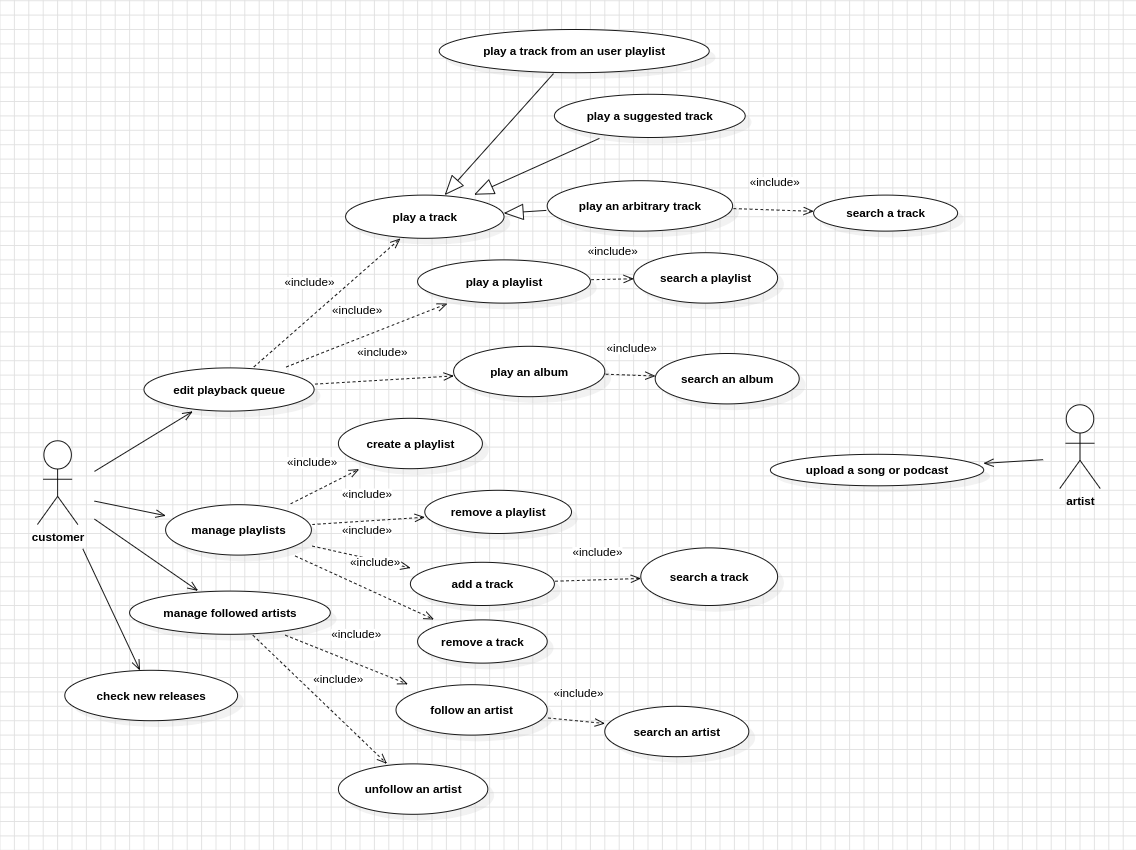
\includegraphics[scale=0.3]{usecase02}

\section{Scelte di progetto}

Abbiamo scelto di strutturare il progetto creando una divisione tra domain model, business logic e data
access objects.
\begin{itemize}
  \item
    Il package  \textbf{domainmodel} definisce le classi che simboleggiano gli elementi con cui l'utente
    interagisce.
  \item
    il package \textbf{businesslogic} descrive le modalità e le possibilità di interazione che l'utente
    ha con tali oggetti.
  \item
    il \textbf{dao} garantisce la persistenza di alcuni oggetti all'interno dell'applicazione.

   \end{itemize}
    
\section{Documentazione}

\section{Test}   
\end{document}
